\subsection{IIS通信协议}
\subsubsection{IIS概述}
I2S = Inter-IC Sound = Integrated Interchip Sound = IIS,是飞利浦在1986年定义(1996年修订)的数字音频传输标准,用于数字音频数据在系统内器件之间传输,例如编解码器CODEC、DSP、数字输入/输出接口、ADC、DAC和数字滤波器等。其与IIC无关联。

\subsubsection{IIS硬件结构}
IIS是个相对来说简单的接口协议,没有地址和片选机制。在总线上,只能同时存在一个主设备和发射设备;提供时钟的设备为主设备,可以是发射设备也可以是接收设备,或者是协调两者的其他控制设备。在高端应用场合中,CODEX经常作为主设备以便精确控制IIS的数据流。

%=============================================================%
%                       插入一张图片                          %
%=============================================================%
\begin{figure}[H]
\centering
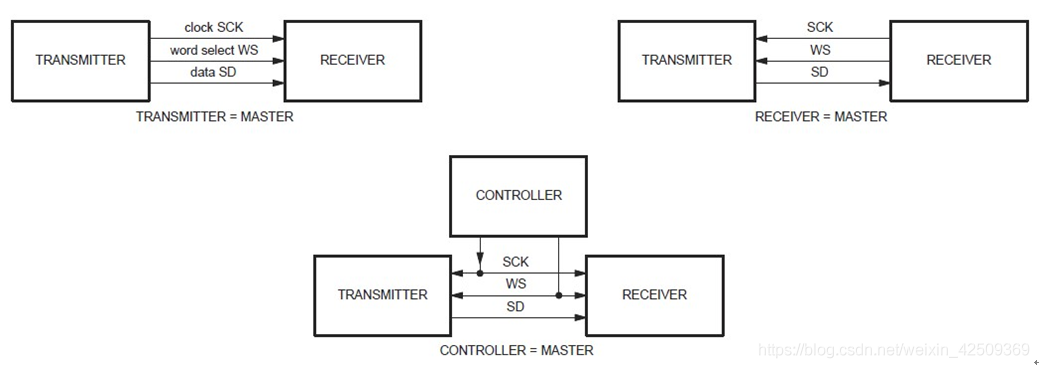
\includegraphics[scale=0.3]{iis_topo.png}
\caption{IIS硬件TOPO结构}
\end{figure}

IIS协议定义三根信号线:时钟信号SCK、数据信号SD和左右声道选择信号WS。
\begin{itemize}
\item WS:声道选择信号,表明数据发送端所选择的声道: WS=0,表示选择左声道,WS=1,表示选择右声道,同时也叫帧时钟,等于声音的采样率。
\item SCK:模块内的同步信号,从模式时由外部提供,主模式时由内部产生。
\item SD:串行数据,以二进制补码形式在数据线上传输;在WS变化后的第一个SCK脉冲,先传输最高位(MSB, Most Significant Bit)。
\end{itemize}

\subsubsection{IIS工作模式}
IIS的操作模式分为三种:标准IIS模式、左对齐模式和右对齐模式。
\begin{itemize}
\item 标准IIS模式(Phillips Standard)

IIS模式是标准左对齐格式再延迟一个时钟位变化来的,时序如下所示:
\begin{figure}[H]
\centering
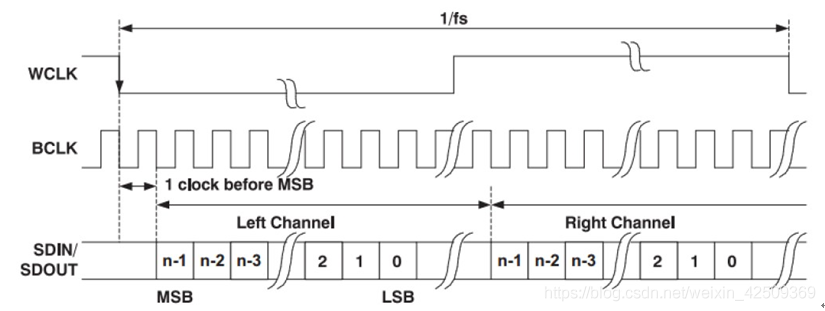
\includegraphics[scale=0.4]{iis_starndar_mode.png}
\caption{标准IIS模式}
\end{figure}
左右通道的数据MSB均是在WS变化后第二个SCK/BCLK上升沿有效。

\item 左对齐模式(Left Justified Standard)

标准左对齐格式的数据的MSB没有相对于BCLK延迟一个时钟。左对齐格式的左右声道数据的MSB在WS边沿变化后SCK/BCLK的第一个上升沿有效。具体如下图所示:
\begin{figure}[H]
\centering
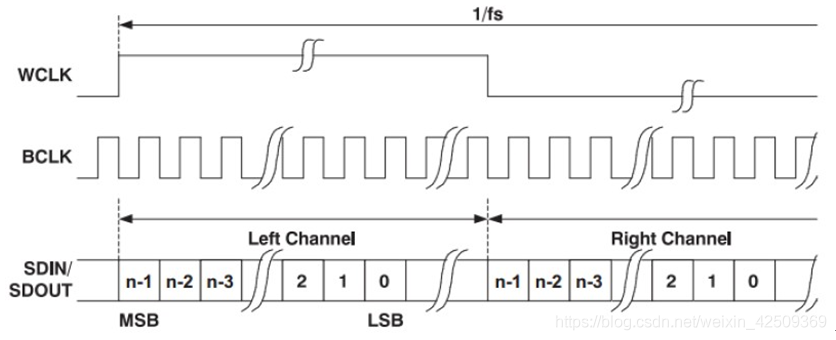
\includegraphics[scale=0.4]{iis_left_mode.png}
\caption{IIS左对齐模式}
\end{figure}
支持16~32bit字长格式;

\item 右边对齐模式(Right Justified Standard)

也叫日本格式,sony格式,具体对齐方式如下图所示:
\begin{figure}[H]
\centering
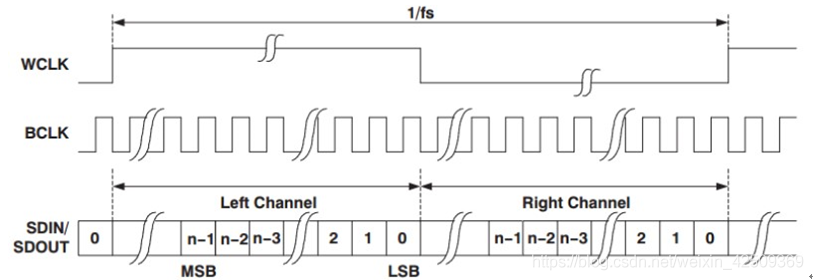
\includegraphics[scale=0.4]{iis_right_mode.png}
\caption{IIS右对齐模式}
\end{figure}
接收设备必须事先知道待传数据的字长。

\end{itemize}

\begin{messagebox}
注意左右对齐模式的WS时钟高电平为左声道,低电平为右声道,刚好与标准IIS相反。
\end{messagebox}

\subsubsection{IIS时钟频率计算}
SCK = 采样率(48K、44.1K、16K等) x  字长(16bit、24bit、32bit) x 2(左右两通道);MCLK/SCK =  384 、256 等需要参考手册说明支持哪种;


\subsubsection{ES9018芯片IIS通信实例}
ES9018芯片数据手册\myurlfootnote{https://pan.baidu.com/s/123GuxBl2Uig3Jy3Jfp4MTw}{链接},提取码:ix8r。\newline
ES9018芯片IIS只支持64SCLK/Frame,数据位宽支持32/24/20/16bit模式,时序如下:
\begin{figure}[H]
\centering
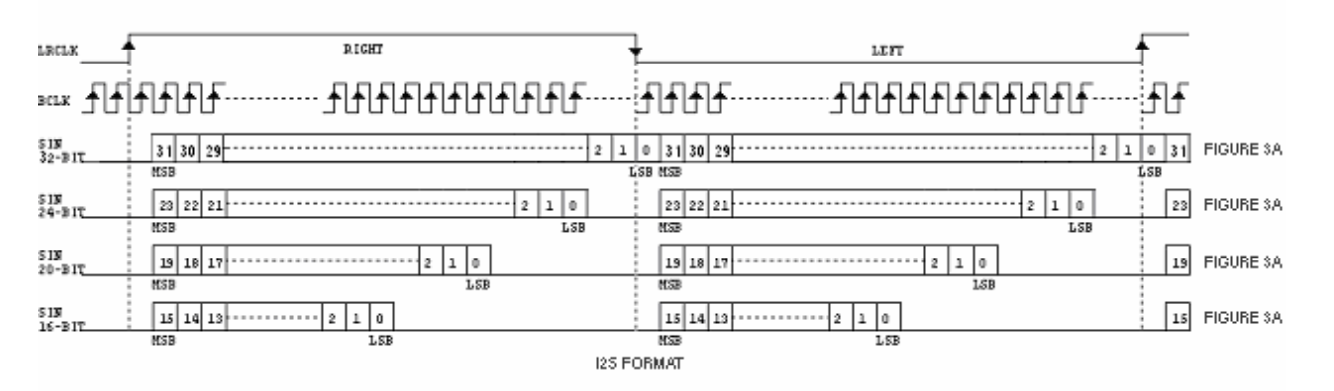
\includegraphics[scale=0.4]{ES9018_IIS.png}
\caption{ES9018 IIS时序图}
\end{figure}
由时序图可知,各种数据位宽都统一使用64SCK/Frame模式,如果主机传输位宽少于ES9018的数据位宽,低位应该会补全0或者全1,不同接收模式可通过IIC通信配置,寄存器定义如下:
\begin{figure}[H]
\centering
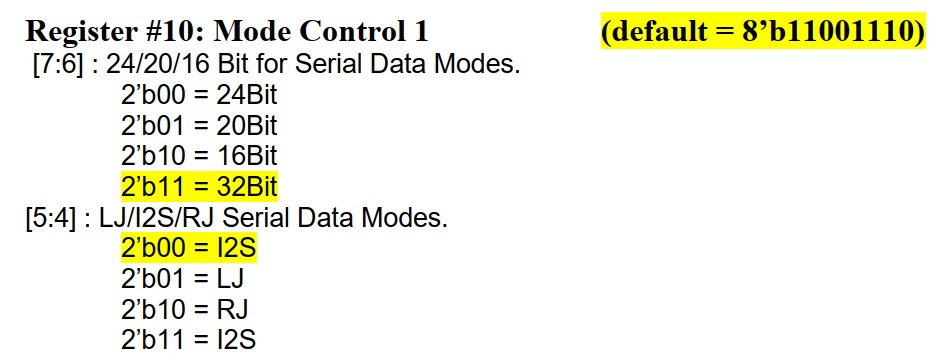
\includegraphics[scale=0.4]{ES9018_IIS_default_config.jpg}
\caption{ES9018 IIS模式配置}
\end{figure}
ES9018 IIS默认模式是标准IIS,位宽为32bit模式,默认采样率为44.1K。
\begin{figure}[H]
\centering
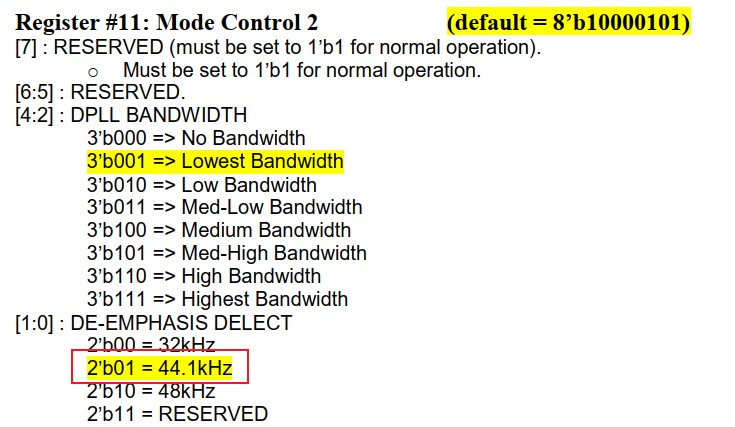
\includegraphics[scale=0.4]{ES9018_IIS_sr_config.jpg}
\caption{ES9018默认采样率配置}
\end{figure}
ES9018硬件标号标定如下:
\begin{figure}[H]
\centering
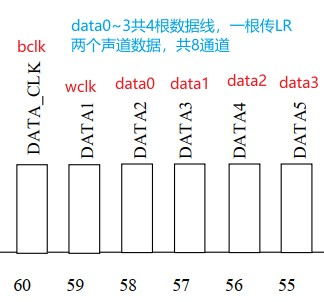
\includegraphics[scale=1]{ES9018_HW_IIS_PIN.jpg}
%\caption{ES9018硬件IIS引脚}
\end{figure}
\begin{figure}[H]
\centering
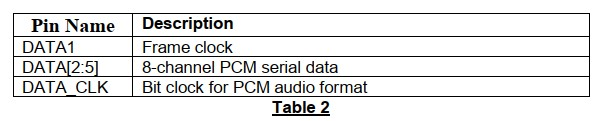
\includegraphics[scale=1]{ES9018_HW_IIS_PIN2.jpg}
\caption{ES9018硬件IIS引脚}
\end{figure}

调试遇到问题:
\begin{itemize}
\item 用32clk/frame传输时数据,传输1k频率,44.1K采样率的数据,ES9018 DAC数据信号会变为44.1K的正弦波信号;
\item 我们Audio Link需要需要用64clk/frame模式,位宽可以为16bit,中断填数需要注意左右声道数据交错,否则会出现不可预料的问题;
\end{itemize}

\subsubsection{一些问题解答}
\begin{itemize}
    \item \emphasizebox{384, 512fs}代表什么意思?\newline
        256fs中“fs” 就是表示audio sampling frequency, 表示在一个LR周期中BCLK的个数,比如;数据是32bit位宽,2个通道,那么fs就是32 x 2 = 64fs,可以理解为一帧有多少个sclk, fs参数结合采样率(LRCLK)可以算出BCLK,BCLK与MCLK存在分频关系,这个关系与实际通信芯片有关;
\end{itemize}
